\documentclass[11pt,nocut]{article}

\usepackage{../latex_style/packages}
\usepackage{../latex_style/notations}
%\externaldocument{../lecture_02/lecture_02}
\externaldocument{../lecture_07/lecture_07}


\title{\vspace{-2.0cm}%
	Optimization and Computational Linear Algebra for Data Science\\
Lecture 10: Linear regression}
\author{Léo \textsc{Miolane} \ $\cdot$ \ \texttt{leo.miolane@gmail.com}}
\date{\today}

\begin{document}
\maketitle
\textbf{Warning:}
\emph{This material is not meant to be lecture notes. It only gathers the main concepts and results from the lecture, without any additional explanation, motivation, examples, figures...
}


\section{Least squares}

Assume that we are given point $a_i = (a_{i,1}, \dots, a_{i,d}) \in \R^d$ with labels $y_i \in \R$ for $i=1 \dots n$.
We aim at finding a vector $x\in\R^d$ such that
$$
y_i \simeq \langle a_i, x \rangle = \sum_{j=1}^d a_{i,j} x_j, \qquad \text{for} \ \ i=1 \dots n.
$$
If we denote by $A$ the $n \times d$ matrix whose rows are $a_1, \dots, a_n$, i.e.\ $A_{i,j} = a_{i,j}$, we are looking for some $x$ such that $Ax \simeq y$.
\\

In general, solutions to $Ax=y$ may not exist: there is no reason for $y$ to belong to $\Im(A)$, especially when $n > d$. (Exercise: why?)
Moreover, the measurements may contain some noise.
Therefore one is rather interested by solving
\begin{equation}\label{eq:least_squares}
	\text{minimize} \quad \| Ax - y \|^2, \quad \text{with respect to} \quad x \in \R^d.
\end{equation}
The function $f: x \mapsto \|Ax - y\|^2$ is convex (Exercise: why?) and differentiable. Hence
$x$ is solution of \eqref{eq:least_squares} if and only if $\nabla f (x) = 0$. Compute
$$
f(x) = (Ax - y)^{\sT}(Ax - y) = x^{\sT} A^{\sT} A x - 2 y^{\sT} A x + \|y\|^2.
$$
Hence $\nabla f(x) = 2 A^{\sT} A x - 2 A^{\sT} y$. We conclude
$$
x \ \ \text{is solution of} \ \ \eqref{eq:least_squares} \qquad
\Longleftrightarrow
\qquad A^{\sT} A x = A^{\sT} y.
$$
If $A^{\sT} A$ is invertible there is a unique minimizer $x^* = (A^{\sT} A)^{-1} A^{\sT} y$.
In the general case, we see that the solutions of \eqref{eq:least_squares} are the solutions of the linear system $A^{\sT} A x = A^{\sT} y$. 
Let $A=U\Sigma V^{\sT}$ be the singular value decomposition of $A$. Using the SVD, the linear system can be rewritten as
\begin{equation}\label{eq:simpSVD}
V \Sigma^{\sT} \Sigma V^{\sT} x = V \Sigma^{\sT} U^{\sT} y
\qquad
\text{which is equivalent to}
\qquad
\Sigma^{\sT} \Sigma V^{\sT} x = \Sigma^{\sT} U^{\sT} y
\end{equation}
because $V$ is invertible (recall that $V$ is orthogonal). We will now introduce:

\begin{definition}[Moore-Penrose pseudo-inverse]
	The matrix $A^{\dagger} \defeq V \Sigma' U^{\sT}$ is called the (Moore-Penrose) pseudo-inverse of $A$, where $\Sigma'$ is the $d \times n$ matrix given by 
	$$
	\Sigma'_{i,i} =
	\begin{cases}
		1 / \Sigma_{i,i} & \text{if} \ \Sigma_{i,i} \neq 0, \\
		0 & \text{otherwise},
	\end{cases}
	$$
	and $\Sigma'_{i,j} = 0$ for $i \neq j$.
\end{definition}

Now, one can check that $x = A^{\dagger}y$ is a solution of \eqref{eq:simpSVD}:
$$
\Sigma^{\sT} \Sigma V^{\sT} A^{\dagger} y =
\Sigma^{\sT} \Sigma \Sigma' U^{\sT} y =
\Sigma^{\sT} U^{\sT} y.
$$
Hence, the set of solutions of the linear system $A^{\sT} A x = A^{\sT} y$ is $A^{\dagger} y + \Ker(A^{\sT}A)$. Notice now that (exercise!) we have $\Ker(A^{\sT} A) = \Ker(A)$.
We conclude:

\begin{proposition}[Least squares]\label{prop:least_squares}
	The set of solution of the minimization problem $\min_{x \in \R^n} \|Ax - y\|^2$ is
	$$
	A^{\dagger} y + \Ker(A).
	$$
\end{proposition}

We deduce:
\begin{corollary}\label{cor:linear_system}
	The set of solution of the linear system $Ax = y$ is
	\begin{itemize}
		\item $\emptyset$ if $y \not\in \Im(A)$.
		\item $A^{\dagger}y + \Ker(A)$ otherwise.
	\end{itemize}
\end{corollary}


\section{Penalized least squares: Ridge regression and Lasso}

When $\Ker(A) \neq \{0\}$ the least squares problem \eqref{eq:least_squares} has an infinite number of solutions: which one should we pick?

\subsection{Ridge regression}

The Ridge regression adds a $\ell_2$ penalty to the least square problem in order to ``select'' a solution of smaller norm, and minimizes
\begin{equation}\label{eq:ridge}
	\min_{x \in \R^d} \Big\{ \| Ax - y \|^2 + \lambda \|x\|^2 \Big\},
\end{equation}
for some penalization parameter $\lambda >0$.
\begin{exercise}
	Show that \eqref{eq:ridge} admits a unique solution given by
	$$
	x^{\rm Ridge} = (A^{\sT} A + \lambda \Id)^{-1} A^{\sT} y.
	$$
\end{exercise}

\subsection{Lasso}

The Lasso adds a $\ell_1$ penalty to the least square problem, and minimizes
\begin{equation}\label{eq:lasso}
\frac{1}{2} \| Ax - y \|^2 + \lambda \|x\|_1,
\end{equation}
for some penalization parameter $\lambda >0$.
Here, the cost function is not strictly convex in general, hence there may be multiple minimizers. However, in many situations (for instance if the entries of $A$ are drawn from a continuous probability distribution) the minimizer $x^{\rm Lasso}$ will be unique \cite{tibshirani2013lasso}.
\\

The Lasso has the wonderful property of \emph{feature selection}: the solution $x^{\rm Lasso}$ of \eqref{eq:lasso} is likely to be \emph{sparse} (many coordinates $x^{\rm Lasso}_j$ will be set to $0$).
In words, the Lasso estimator discards the ``useless features'' by setting its corresponding coefficient to $0$. 
This is particularly nice for the interpretability of the results: in many application, each data point $a_i$ has an enormous number of features ($d$ very large), but only a small number of them are useful to predict the label $y_i$.
\\

We will now give some intuition on this phenomena. First, we have the following

\begin{lemma}\label{lem:ball}
	Let $x^{\rm Lasso}$ be a minimizer of the Lasso cost function \eqref{eq:lasso} and let $r=\|x^{\rm Lasso}\|_1$. Then $x^{\rm Lasso}$ is a solution to
	$$
	\text{minimize} \quad \frac{1}{2} \|Ax-y\|^2 \quad
	\text{subject to} \quad \|x\|_1 \leq r.
	$$
\end{lemma}
\begin{proof}
	By contradiction, assume that there exists $x \in \R^d$ such that $\|Ax -y\|^2 < \|Ax^{\rm Lasso}-y\|^2$ and $\|x\|_1 \leq r = \|x^{\rm Lasso}\|_1$. Then
	$$
\frac{1}{2} \| Ax - y \|^2 + \lambda \|x\|_1 
< 
\frac{1}{2} \| Ax^{\rm Lasso} - y \|^2 + \lambda \|x^{\rm Lasso}\|_1,
$$
which contradicts the fact that $x^{\rm Lasso}$ is a minimizer of \eqref{eq:lasso}.
\end{proof}
\\

Lemma \ref{lem:ball} tells us that a solution $x^{\rm Lasso}$ of the Lasso problem is a minimizer of the quadratic function $\|Ax-y\|^2$ on the $\ell_1$-ball $B_{\ell_1}(r) = \{x \, | \, \|x\|_1 \leq r\}$.

\begin{figure}[h!]
	\begin{center}
		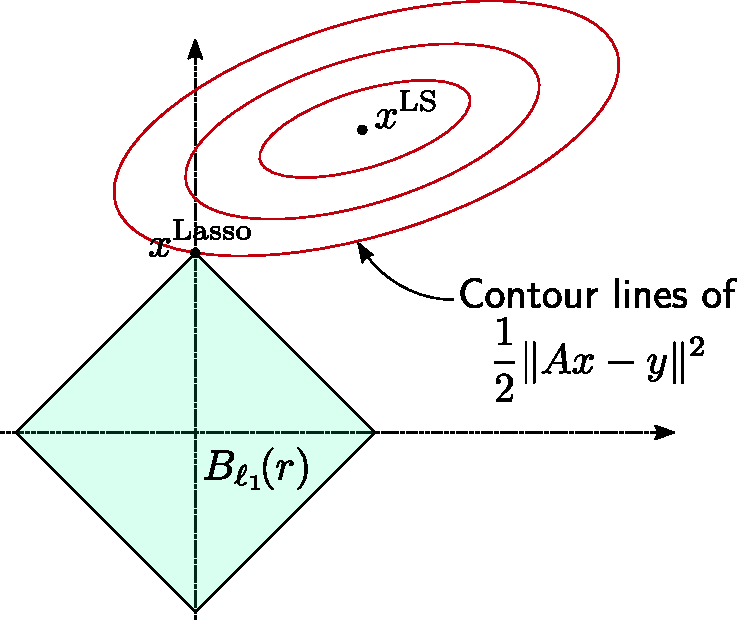
\includegraphics[width=0.6\linewidth]{lasso.pdf}
	\end{center}
	\caption{}
	\label{fig:lasso}
\end{figure}
This is illustrated on Figure~\ref{fig:lasso} above. The Lasso solution $x^{\rm Lasso}$ is the first point at which the elliptical contour lines of the function $\frac{1}{2}\|Ax-y\|^2$ hit the $\ell_1$-ball $B_{\ell_1}(r)$. Observe that the $\ell_1$-ball has corners: $x^{\rm Lasso}$ is therefore very likely to be at one of these corners which is a point where many coordinates are set to zero. Hence, the $\ell_1$ penalization tends to produce sparse solutions.
\\

\paragraph{Lasso for orthonormal design.}
We will show by a computation below that the $\ell_1$ penalization induces sparsity, on a toy example.
In general there is no closed form formula for the Lasso estimator. It is however possible to derive one in the case where the matrix $A$ has orthonormal columns: $A^{\sT} A = \Id$. 
The least square estimator is then given by $x^{\rm LS} = A^{\sT} y$ and the Lasso cost function becomes
\begin{equation}\label{eq:lasso_o}
\frac{1}{2} \| Ax - y \|^2 + \lambda \|x\|_1 
= \frac{1}{2} \|x\|^2 - \langle x^{\rm LS}, x \rangle + \frac{1}{2} \|y\|^2 + \lambda \|x\|_1.
\end{equation}
The minimizer of \eqref{eq:lasso_o} is therefore the minimizer of
$$
\frac{1}{2} \|x\|^2 - \langle x^{\rm LS}, x \rangle + \lambda \|x\|_1
=
\sum_{j=1}^d \frac{x_j^2}{2} - x^{\rm LS}_j x_j + \lambda |x_j| 
=
\sum_{j=1}^d f_{x_j^{\rm LS}}(x_j),
$$
where $f_{x_0}(x) \defeq \frac{1}{2}x^2 - x_0 x + \lambda |x|$.

\begin{exercise}
	Show that the function $f_{x_0}$ admits a unique minimizer given by
	$$
	x^* = \eta(x_0; \lambda),
	$$
	where $\eta$ denotes the ``soft-thresholding'' function:
	$$
	\eta(x_0;\lambda) = 
	\begin{cases}
		x_0-\lambda & \text{if} \quad x_0 \geq \lambda \\
		0 & \text{if} \quad -\lambda \leq x_0 \leq \lambda \\
		x_0 + \lambda & \text{if} \quad x_0 \leq -\lambda.
	\end{cases}
	$$
\end{exercise}
\vspace{2mm}

We conclude that the Lasso estimator is given by
$$
x^{\rm Lasso}_{j} = \eta\big(x_j^{\rm LS}; \lambda\big) \qquad \text{for} \quad j=1, \dots, d.
$$
This formula confirms the intuition given by Figure \ref{fig:lasso}: the Lasso estimator translates the coefficients of the least-square solution by $\lambda$, truncating at $0$.


\section{Norms for matrices}

Before looking at low-rank matrix estimation and matrix completion, we need to look at different norms we can have for matrices. Recall that $\R^{n \times m}$, the set of $n \times m$ matrices, is a vector space (of dimension $nm$).
\\

\paragraph{The Frobenius norm.} The most obvious norm to consider is the equivalent of the $\ell_2$ norm, called the Frobenius norm:
\begin{definition}[Frobenius norm]
	The Frobenius norm of a matrix $A \in \R^{n \times m}$ is defined as
	$$
	\|A\|_F = \sqrt{\sum_{i=1}^n \sum_{j=1}^m A_{i,j}^2}. 
	$$
\end{definition}

\begin{remark}
	The Frobenius norm is the norm induced by the following inner-product:
	$$
	\langle A,B \rangle_{F} = \Tr(A^{\sT}B) = \sum_{i=1}^n\sum_{j=1}^m A_{i,j} B_{i,j}, \qquad \text{for} \ \ A,B \in \R^{n \times m}.
	$$
\end{remark}

\begin{proposition}
	Let $A \in \R^{n \times n}$ and let $\sigma_1, \dots, \sigma_{\min(n,m)}$ be the singular values of $A$. Then
	$$
	\|A\|_F = \sqrt{\sum_{i=1}^{\min(n,m)} \sigma_i^2}.
	$$
\end{proposition}


\paragraph{The spectral norm.} Another extremely common norm for matrices is the spectral norm, also called the operator norm:

\begin{definition}[Spectral norm]
	The spectral norm of a matrix $A \in \R^{n \times m}$ is defined as the maximal singular value of $A$:
	$$
	\|A\|_{\rm Sp} = \max_{\substack{x \in \R^m \\ \|x\|=1}} \|Ax\|.
	$$
\end{definition}
\begin{proposition}
	$$
	\|A\|_{\rm Sp} = \sigma_1(A),
	$$
	where $\sigma_1(A)$ denotes the largest singular value of $A$.
\end{proposition}

\paragraph{The nuclear norm.} We have seen above that the Frobenius norm of a matrix correspond to the $\ell_2$ norm of its singular values and that the spectral norm correspond to the infinity norm of the singular values. The nuclear norm is simply the $\ell_1$ norm of its singular values:
\begin{definition}[Nuclear norm]
	Let $A \in \R^{n \times m}$ and let $\sigma_1, \dots, \sigma_{\min(n,m)}$ be the singular values of $A$. The nuclear norm of $A$ is defined as:
	$$
	\|A\|_* = \sum_{i=1}^{\min(n,m)} \sigma_i.
	$$
	
\end{definition}

\section{Low-rank matrix estimation and matrix completion}



\section*{Further reading}

Chapter 3 of \cite{friedman2001elements} is an excellent reference for linear regression.

\vspace{1cm}
\centerline{\pgfornament[width=7cm]{71}}


\bibliographystyle{plain}
\bibliography{../references.bib}
\end{document}
